\documentclass{article}
\RequirePackage[a4paper]{geometry}
\geometry{top=25mm,bottom=25mm,left=25mm,right=25mm}
\usepackage{mathptmx,graphicx}
\usepackage{microtype}
\setlength{\emergencystretch}{1.5em}
\usepackage[dvipsnames]{xcolor}
\usepackage[numbers,sort&compress]{natbib}
\usepackage{hyperref}
\usepackage[labelfont=bf]{caption}
\usepackage{amssymb}
\usepackage{amsmath}
\usepackage{booktabs}
\graphicspath{{figures/}}
\bibliographystyle{unsrt}

% Supplementary numbering: Section S1, Eq. (S1), Fig. S1, Table S1
\renewcommand{\thesection}{S\arabic{section}}
\renewcommand{\theequation}{S\arabic{equation}}
\renewcommand{\thefigure}{S\arabic{figure}}
\renewcommand{\thetable}{S\arabic{table}}
% Open points for the authors
\newcommand{\note}[1]{\textcolor{red}{[#1]}}

\begin{document}

\begin{center}
{\Large\bfseries Supplementary Material\par}
\vspace{1.5ex}
{\large\bfseries Breaking the Phase-Ambiguity Limit: Reference-less 3D Vectorial Transmission-Matrix Retrieval in Multimode Fibers\par}
\vspace{2ex}
{\bfseries Dvir Marsh, Lior Fridman, Shie Mannor, Guy Bartal\par}
\end{center}
\vspace{2ex}

%------------------------------------------------------------------------------
\section{Guided-mode basis}
\label{sec:modes}
The modal basis consists of the guided vector modes of a step-index fiber.
The fiber has core radius $a=25\,\mu$m, core index $n_1=1.457$, and $\mathrm{NA}=0.22$, and is operated at $\lambda=632.8$\,nm.
Its normalized frequency is $V=k_0a\,\mathrm{NA}=54.61$, with $k_0=2\pi/\lambda$.

We compute the modes in the weak-guidance approximation \cite{fiber_book}.
For each azimuthal order $l\geq0$, the transverse parameter $u$ of the $\mathrm{LP}_{l,m}$ group is the $m$-th root of
\begin{equation}
\label{eq:dispersion}
\frac{J_l(u)}{u\,J_{l-1}(u)}=-\frac{K_l(w)}{w\,K_{l-1}(w)},\qquad w=\sqrt{V^2-u^2},
\end{equation}
where $J_l$ and $K_l$ are the Bessel and modified Bessel functions, with $J_{-1}=-J_1$ and $K_{-1}=K_1$.
The propagation constant of the group is $\beta=\sqrt{k_0^2n_1^2-u^2/a^2}$.
Equation~\eqref{eq:dispersion} has 386 guided solutions for our fiber: 18 with $l=0$, 17 with $l=1$, and 351 with $l\geq2$.

Each solution contributes the vector modes of its group.
A group with $l=0$ contains the two $\mathrm{HE}_{1,m}$ modes.
A group with $l=1$ contains $\mathrm{TE}_{0,m}$, $\mathrm{TM}_{0,m}$, and the two $\mathrm{HE}_{2,m}$ modes.
A group with $l\geq2$ contains the two $\mathrm{EH}_{l-1,m}$ and the two $\mathrm{HE}_{l+1,m}$ modes.
The two modes of each HE or EH pair have opposite azimuthal dependence, $e^{\pm in\varphi}$, where $n$ is the azimuthal order of the vector mode.
The total is $M=2\times18+4\times(17+351)=1508$ modes: 772 HE, 702 EH, 17 TE, and 17 TM.

The transverse profiles $(\psi_{l,x},\psi_{l,y})$ of Eq.~(1) of the main text follow from the analytical field expressions of Ref.~\cite{fiber_book}.
We evaluate them in the core and in the cladding with the parameters $u$ and $w$ of the group.
Each profile is sampled on the $128\times128$ grid of the image plane (Section~\ref{sec:experiment}) and normalized to unit power.
The straight-fiber prior $T_0$ of the Methods uses the propagation constants $\beta$ with $L=1$\,m.

In this approximation, all vector modes of a group share the radial profile of their LP group.
The modes of a group therefore span the scalar $\mathrm{LP}_{l,m}$ profiles, $e^{\pm il\varphi}$, multiplied by both polarization components.
Section~\ref{sec:polframe} relies on this property.

%------------------------------------------------------------------------------
\section{Experimental and data-processing details}
\label{sec:experiment}
\paragraph{Input side.}
The SLM (Meadowlark Optics, $1920\times1200$ pixels) has a pixel pitch of $8\,\mu$m.
We use a region of $640\times640$ pixels, grouped into $128\times128$ macro-pixels of $5\times5$ pixels each.
The relay L1--L2 demagnifies the SLM plane by $150/400$, so this region is $1.92$\,mm wide in the back focal plane of O1.
The NA-limited disk in that plane has a diameter of $2\,\mathrm{NA}\,f=1.76$\,mm, where $f=4$\,mm is the focal length of the objective.

\paragraph{Detection and frame processing.}
BS2 is a pellicle beam splitter (Thorlabs BP245B1) at $45^\circ$ incidence.
The image-plane camera is on its reflected port, and the Fourier-plane camera is on its transmitted port.
Both cameras (Basler daA1920-160um) have a pixel pitch of $3.45\,\mu$m.
The image-plane camera records the output facet at a magnification of 50, which corresponds to 69\,nm per camera pixel.
We crop a square of $798\times798$ camera pixels centered on the core and resize it to $128\times128$ pixels by bilinear interpolation.
The side of this square is $2.2a$, so one pixel of the resized frame corresponds to $0.430\,\mu$m on the facet.
The Fourier-plane camera samples the back focal plane of O2 with the same pixel pitch.
We crop a square of $562\times562$ camera pixels, of side $2.2\,\mathrm{NA}\,f$, and resize it to $128\times128$ pixels.
One pixel of this frame corresponds to $15.1\,\mu$m in the back focal plane.
In both resized frames, the region $\Omega_F$ of the main text is a centered disk of radius $58.1$ pixels.
It covers the core in the image plane and the NA-limited disk in the Fourier plane.

\paragraph{Acquisition.}
After each SLM update we wait 60\,ms, and then both cameras expose simultaneously.
The probe patterns are $6032=4M$ phase masks that were designed once, in advance.
Their phases were optimized with the calibrated input side of the forward model, so that the input modal vectors $\mathbf{z}_{\mathrm{in}}$ excite the guided modes evenly and overlap little with one another.
The participation ratio of the modal covariance $Z_{\mathrm{in}}Z_{\mathrm{in}}^{\dagger}$ is 744 for these masks, compared with 431 for random phase masks.
The data of the time benchmark (Fig.~6 of the main text) consist of two recordings of these patterns.
The first set was recorded before the fiber was displaced and serves the joint fit (Section~\ref{sec:jointfit}).
The second set was recorded after a motorized stage displaced a point along the fiber by 5\,mm.
The displacement changed the bend of the fiber, while both facets stayed fixed.
The fast ADMM retrieval uses random subsets of this second set.
The demonstrations of Figs.~3--5 of the main text use a separate recording of the same patterns.

%------------------------------------------------------------------------------
\section{Joint fit of the TM and the optics}
\label{sec:jointfit}
The joint fit minimizes the loss $L_{\mathrm{PCC}}$ of the Methods with the Adam optimizer.
The trainable parameters are the following.
\begin{itemize}
\item The TM, $T\in\mathbb{C}^{M\times M}$.
\item The complex SLM mask $A(x,y)$ on the $128\times128$ macro-pixel grid.
\item The polarization angle $\theta_{\mathrm{in}}$ of the incident field and a polarization rotation after the SLM.
\item Four sets of eight Zernike coefficients (Noll indices 4--11). The sets act before and after the input objective, in the image plane, and in the Fourier plane.
\item Scale and offset parameters of the three numerical Fourier transforms of the model. Each transform has two scale factors and four center offsets.
\item For the test of Section~\ref{sec:polframe} only: the camera weight $b$ of Eq.~\eqref{eq:camweights}, parameterized as $b=\tanh\beta$.
\end{itemize}
The three transforms connect the SLM to the input facet, the image plane to the Fourier plane, and the Fourier plane back to the image plane.
The TM starts from the straight-fiber prior $T_0$; the other initial values, the learning rates, and the batch sizes are listed in the published code.
We train for 100 epochs.
In each case, $95\%$ of the patterns are used for training and $5\%$ are held out.
For the dataset of Section~\ref{sec:polframe}, the PCC between predicted and measured intensities on the held-out patterns is $0.913$ in the image plane and $0.929$ in the Fourier plane.
After the fit, the operators $Z_{\mathrm{in}}$ and $P_{c,p}$ are computed once from the fitted parameters and kept fixed.

%------------------------------------------------------------------------------
\section{Closed-form TM update of the fast ADMM}
\label{sec:tmupdate}
Step~1 of Algorithm~1 minimizes
\begin{equation}
\label{eq:objective}
f(T)=\sum_{c,p}\kappa_p\left\|P_{c,p}\,T\,Z_{\mathrm{in}}-V_{c,p}\right\|_F^2,\qquad V_{c,p}=U_{c,p}-\Lambda_{c,p},
\end{equation}
where $P_{c,p}\in\mathbb{C}^{N\times M}$, $Z_{\mathrm{in}}\in\mathbb{C}^{M\times K}$, and $V_{c,p}\in\mathbb{C}^{N\times K}$ for $N$ pixels per plane and $K$ SLM patterns.
The objective is quadratic in $T$, and its gradient with respect to $T^*$ is
\begin{equation}
\frac{\partial f}{\partial T^*}=\sum_{c,p}\kappa_p\,P_{c,p}^{H}\left(P_{c,p}\,T\,Z_{\mathrm{in}}-V_{c,p}\right)Z_{\mathrm{in}}^{H}.
\end{equation}
Setting the gradient to zero gives the normal equations
\begin{equation}
\label{eq:normal}
G\,T\,C=B\,Z_{\mathrm{in}}^{H},\qquad
G=\sum_{c,p}\kappa_p\,P_{c,p}^{H}P_{c,p},\quad
C=Z_{\mathrm{in}}Z_{\mathrm{in}}^{H},\quad
B=\sum_{c,p}\kappa_p\,P_{c,p}^{H}V_{c,p}.
\end{equation}
Their solution is
\begin{equation}
\label{eq:closedform}
T=G^{+}\,B\,Z_{\mathrm{in}}^{H}\,C^{+},
\end{equation}
where $^{+}$ denotes the Moore--Penrose pseudo-inverse.

The matrices $G$ and $C$ are $M\times M$ and do not change during the iterations.
$G$ depends only on the modal projections and the plane weights, and $C$ depends only on the SLM patterns.
We therefore compute $G^{+}$ and $C^{+}$ once, discarding singular values below $10^{-4}$ of the largest one.
Each iteration then requires only the matrix $B$ and the products of Eq.~\eqref{eq:closedform}.
On the workstation of the main text, one iteration takes $0.13$--$0.30$\,s for $K=1.2M$ to $3M$.

The pseudo-inverse is needed because $C$ is rank deficient.
The SLM modulates one input polarization, so the vectors $\mathbf{z}_{\mathrm{in}}$ span only about half of the input modal space.
Equation~\eqref{eq:closedform} then returns the minimum-norm solution, which is determined on the subspace that the SLM patterns excite.
This subspace is sufficient to predict the output field of any SLM pattern.
Before the iterations, the intensities are divided by their global mean and $Z_{\mathrm{in}}$ by its largest magnitude, for numerical stability in single precision.

%------------------------------------------------------------------------------
\section{Computing SLM patterns from the retrieved TM}
\label{sec:slm}
All SLM patterns in the main text are computed by gradient-based optimization through the forward model.
The TM and the fitted parameters of the optics are held fixed.
The optimization variable is the phase $\Phi$ of the $128\times128$ macro-pixels, initialized with independent uniform values in $[0,2\pi)$.
We use the Adam optimizer with a learning rate of $0.1$ for 150 iterations, and 90 iterations in the time benchmark.
The resulting phase is wrapped to $[0,2\pi)$, quantized to 256 levels, and replicated over the $5\times5$ SLM pixels of each macro-pixel.
The targets differ only in the objective that is maximized.

\paragraph{Single focus.}
For a target pixel $\mathbf{r}_t$ in plane $p$, we maximize
\begin{equation}
\label{eq:focusobj}
F_p(\mathbf{r}_t)=\frac{\langle I_{\mathrm{pred},p}\rangle_{W(\mathbf{r}_t)}}{\langle I_{\mathrm{pred},p}\rangle_{\Omega_F\setminus W(\mathbf{r}_t)}},
\end{equation}
where $W(\mathbf{r}_t)$ is a window of at most $3\times3$ pixels centered on the target.
The objective differs from the reported PBR, which is evaluated on the brightest pixel of the measured focus (Section~\ref{sec:pbr}).

\paragraph{Several foci.}
For targets $\mathbf{r}_1,\dots,\mathbf{r}_J$, the numerator of Eq.~\eqref{eq:focusobj} is replaced by the mean of the $J$ window averages.
The denominator is the mean over $\Omega_F$ outside all windows.
To equalize the foci, we subtract a penalty $\lambda\,\sigma/\mu$ from the objective.
Here, $\mu$ and $\sigma$ are the mean and the standard deviation of the $J$ window averages.
We use $\lambda=10$ in the image plane and $\lambda=100$ in the Fourier plane.

\paragraph{Extended patterns.}
We maximize the PCC between the predicted intensity and the target image over the full $128\times128$ frame.
The target image occupies the central $64\times64$ pixels of the frame and is zero elsewhere.

\paragraph{Single guided mode.}
We maximize $\sum_k p_k^2$, with $p_k=|w_k|^2/\sum_j|w_j|^2$ the fraction of the output power in mode $k$.
This objective is maximal when all the power is in one mode, but it does not prescribe which mode.
The mode reported in the main text is the one that carries the largest fraction after the optimization.

\paragraph{Two orthogonally polarized foci.}
For targets $\mathbf{r}_A$ and $\mathbf{r}_B$, we maximize the product $F_{x'}(\mathbf{r}_A)\,F_{y'}(\mathbf{r}_B)$.
Each factor is Eq.~\eqref{eq:focusobj} evaluated on the intensity of one polarization component of the predicted field, $|E_{x'}|^2$ or $|E_{y'}|^2$.

%------------------------------------------------------------------------------
\section{Focusing metric and its expected value}
\label{sec:pbr}
\paragraph{Definition.}
The PBR of a measured focus is evaluated on the resized $128\times128$ frame.
$I_{\mathrm{peak}}$ is the brightest pixel within 3 pixels of the target, and $\Omega_T$ is the $3\times3$-pixel window centered on it.
The background region $\Omega_B=\Omega_F\setminus\Omega_T$ contains $N_B=N_F-9$ pixels, where $N_F=10{,}612$ is the number of pixels in $\Omega_F$.

\paragraph{Relation to the enhancement.}
The enhancement is commonly defined as $\eta=I_{\mathrm{peak}}/\langle I\rangle_0$ \cite{focusing_coherent}.
Here, $\langle I\rangle_0$ is the mean intensity at the target for unshaped, random SLM patterns.
The PBR instead divides by the background of the same frame, which has lost the power concentrated in the focus.
Assume that the focus pattern and the random patterns transmit the same power, and that $\langle I\rangle_0$ is uniform over $\Omega_F$.
Power conservation over $\Omega_F$ then gives
\begin{equation}
\label{eq:pbr_eta}
\mathrm{PBR}=\frac{\eta}{1-f_T}\,\frac{N_B}{N_F},
\end{equation}
where $f_T$ is the fraction of the power in $\Omega_F$ that falls inside $\Omega_T$.
The PBR therefore exceeds $\eta$ by the factor $1/(1-f_T)$, and it is not bounded by the limit that applies to $\eta$.
Table~\ref{tab:pbr} lists the three quantities for the single-spot foci of the main text.
For this table, $\langle I\rangle_0$ was approximated by the mean of each focus frame over $\Omega_F$.

\begin{table}[h]
\centering
\caption{\textbf{PBR and enhancement of the single-spot foci} (five targets per plane, mean $\pm$ standard deviation). The last three columns are estimates explained in the text.}
\label{tab:pbr}
\begin{tabular}{lcccccc}
\toprule
Plane & PBR & $\eta$ & $f_T$ & Speckle contrast & $\alpha$ & Expected $\eta$ \\
\midrule
Image & $526\pm71$ & $389\pm39$ & $0.26\pm0.02$ & $0.77$ & $0.28$ & $426$ \\
Fourier & $619\pm101$ & $443\pm52$ & $0.28\pm0.04$ & $0.84$ & $0.18$ & $486$ \\
\bottomrule
\end{tabular}
\end{table}

\paragraph{Expected enhancement with polarization-summed detection.}
For phase-only control of $N_{\mathrm{ch}}$ input channels and a single detected polarization, the expected enhancement is $(\pi/4)(N_{\mathrm{ch}}-1)+1$ \cite{focusing_coherent}.
Our cameras sum both polarization components, and the phases can be aligned for only one component of the field at the target.
Let $1-\alpha$ and $\alpha\leq1/2$ be the fractions of the unshaped mean intensity in the dominant polarization component at the target and in the orthogonal one.
Aligning the phases of the dominant component enhances it, while the orthogonal component keeps its unshaped mean.
The expected enhancement of the summed intensity is then
\begin{equation}
\label{eq:eta_pol}
\eta_{\mathrm{exp}}=\frac{\pi}{4}\,(N_{\mathrm{ch}}-1)(1-\alpha)+1.
\end{equation}
See also Refs.~\cite{shen2016,woo2022}.

The fraction $\alpha$ can be estimated from the probe data without a polarizer.
If the two components are independent, fully developed speckle patterns, the contrast of their sum over the SLM patterns is $\sqrt{1-2\alpha(1-\alpha)}$.
The probe frames of the modal retrieval give a contrast of $0.77$ in the image plane and $0.84$ in the Fourier plane (median over the pixels within 45 pixels of the frame center).
The corresponding estimates are $\alpha=0.28$ and $\alpha=0.18$.
With $N_{\mathrm{ch}}=754$, Eq.~\eqref{eq:eta_pol} gives $\eta_{\mathrm{exp}}=426$ and $486$.
The measured $\eta$ is $91\%$ of these values in both planes.
\note{author check: $\alpha$ is inferred from speckle contrast, not measured with a polarizer. In the Fourier plane the unshaped mean intensity is not uniform over $\Omega_F$ (0.67 to 1.44 of its mean), so $\eta$ referenced to the $\Omega_F$ mean underestimates the local enhancement of the five targets by about 15\%.}

%------------------------------------------------------------------------------
\section{Polarization frame of the retrieved TM}
\label{sec:polframe}

\paragraph{Remaining freedom.}
In the basis of Section~\ref{sec:modes}, the guided modes span the scalar LP profiles multiplied by both polarization components.
A Jones matrix $U$ applied uniformly to the field therefore maps the modal subspace onto itself.
Let $\Psi$ be the matrix that stacks the $x$ and $y$ profiles of all modes.
Then $D(U)=\Psi^{+}(U\otimes\mathbb{1})\Psi$ is the $M\times M$ matrix that represents $U$ in the modal basis.
If $U$ is unitary, it leaves the polarization-summed intensity unchanged in both planes.
The matrices $T$ and $D(U)\,T$ thus predict identical intensities for every SLM pattern.
The retrieval can determine the TM only up to this global unitary matrix.
The laboratory field and the field predicted by the retrieved TM are related by
\begin{equation}
\label{eq:frame}
\mathbf{E}_{\mathrm{lab}}(\mathbf{r})=c\,U\,\mathbf{E}(\mathbf{r}),
\end{equation}
with a complex constant $c$ and the same $U$ at every pixel and in both planes.
The retrieved axes $x'$ and $y'$ correspond to two orthogonal polarization states in the laboratory, which are elliptical in general.
The main text refers to this freedom as a global rotation; a rotation of the axes by an angle $\theta$ is the special case $U=R(\theta)$.
We verified this freedom in simulation with the forward model and the fast ADMM retrieval of the Methods, on a scaled-down fiber with $a=8\,\mu$m and $M=156$ modes.
For each of 20 random TMs, the TM was retrieved from $3M$ polarization-summed, dual-plane intensity patterns.
In every case, the true and predicted fields were related by Eq.~\eqref{eq:frame} with a unitary $U$, and the relative residual was below $10^{-10}$.
The matrix $U$ was not a rotation: the $x'$ state was elliptical, with an ellipticity angle of median magnitude $17^\circ$ (range $2^\circ$ to $36^\circ$).

\paragraph{Polarization-dependent detection.}
The freedom of Eq.~\eqref{eq:frame} requires that both cameras weight the two polarization components equally.
In our setup they do not, because the transmittance and the reflectance of BS2 depend on the polarization.
Let $x$ denote the polarization in the plane of incidence of BS2 and $y$ the perpendicular one.
The image-plane camera records $R_x|E_x|^2+R_y|E_y|^2$ and the Fourier-plane camera records $T_x|E_x|^2+T_y|E_y|^2$, each for the field in its own plane.
Here, $R_{x,y}$ and $T_{x,y}$ are the reflectances and transmittances of BS2.
The rescaling $E_x\to\sqrt{R_x}\,E_x$, $E_y\to\sqrt{R_y}\,E_y$ is a uniform Jones matrix, so the TM can absorb it.
The data therefore determine only the weights of one camera relative to the other, and we write
\begin{equation}
\label{eq:camweights}
I_{\mathrm{im}}=|E_x|^2+|E_y|^2,\qquad I_{\mathrm{F}}\propto(1+b)\,|E_x|^2+(1-b)\,|E_y|^2,\qquad \frac{1+b}{1-b}=\frac{T_x\,R_y}{T_y\,R_x}.
\end{equation}
The loss $L_{\mathrm{PCC}}$ does not depend on the constant of proportionality.
The parameter $b$ is fitted together with the TM (Section~\ref{sec:jointfit}).
The retrieved TM then describes the field with its components scaled by $\sqrt{R_x}$ and $\sqrt{R_y}$.

For $b\neq0$, Eq.~\eqref{eq:camweights} reduces the freedom of Eq.~\eqref{eq:frame}.
A unitary matrix $U$ leaves both intensities unchanged for every field only if it commutes with $\mathrm{diag}(1+b,1-b)$.
It is then diagonal, $U=\mathrm{diag}(e^{i\alpha},e^{i\beta})$.
The retrieved axes $x'$ and $y'$ therefore coincide with the axes $x$ and $y$ of BS2.
Two freedoms remain: the phase $\alpha-\beta$ between the two components, and the exchange of the two labels together with $b\to-b$.
The phase does not affect fields polarized along $x$ or $y$.
It can be measured with a polarizer, as described next.

The manufacturer's typical data for BS2 at $632.8$\,nm are $T_x=72.5\%$, $T_y=48.2\%$, $R_x=27.4\%$, and $R_y=50.2\%$.
They give $(1+b)/(1-b)=2.75$, that is, $b=0.47$.
The typical curves show thin-film fringes with a period of about $50$\,nm, over which $b$ varies between $0.36$ and $0.69$.
The value of an individual pellicle therefore depends on its thickness.

\paragraph{Phase between the two components.}
For $b\neq0$, let $E_x$ and $E_y$ be the Fourier-plane components predicted by the retrieved TM.
The field in front of a polarizer at the Fourier-plane camera is then
\begin{equation}
\label{eq:polfield}
\mathbf{E}_{\mathrm{pol}}=c\left(\sqrt{1+b}\;e^{i\delta}E_x,\ \sqrt{1-b}\;E_y\right),
\end{equation}
with a complex constant $c$ and the remaining phase $\delta=\alpha-\beta$.
This phase includes the retardance of BS2 in transmission, so it refers to the field at this camera.
A polarizer at an angle $a$ from the $x$ axis transmits $I_a=|\cos a\,E_{\mathrm{pol},x}+\sin a\,E_{\mathrm{pol},y}|^2$, which gives
\begin{equation}
\label{eq:Ia}
I_a=g\left[\cos^2\!a\;A+\sin^2\!a\;B+\sin2a\,\left(C\cos\delta-S\sin\delta\right)\right].
\end{equation}
Here, $g=|c|^2$, $A=(1+b)|E_x|^2$, $B=(1-b)|E_y|^2$, and $C+iS=\sqrt{1-b^2}\,E_xE_y^{*}$.
The images $A$, $B$, $C$, and $S$ are computed from the retrieved TM for the displayed SLM pattern.
Equation~\eqref{eq:Ia} is linear in $g\cos\delta$ and $g\sin\delta$, and their coefficient is largest at $a=45^\circ$.
A single image of one speckle pattern at $45^\circ$ therefore determines $\delta$.
We fit
\begin{equation}
\label{eq:phasefit}
I_{45^\circ}(\mathbf{r})=c_0+c_A\,A(\mathbf{r})+c_B\,B(\mathbf{r})+c_C\,C(\mathbf{r})-c_S\,S(\mathbf{r})
\end{equation}
by linear least squares over the pixels of $\Omega_F$, and obtain $\delta=\operatorname{atan2}(c_S,c_C)$.
The constant $c_0$ absorbs a background.
Fitting $A$ and $B$ with separate coefficients absorbs a small error of the polarizer angle.
The images of several SLM patterns can enter the same fit.
The polarizer must be at $45^\circ$ and not at $135^\circ$: the other diagonal changes the result by $180^\circ$.
With a second image at $135^\circ$, the difference $I_{45^\circ}-I_{135^\circ}=2g\left(C\cos\delta-S\sin\delta\right)$ contains neither $A$ and $B$ nor the background.
Once $\delta$ is known, Eq.~\eqref{eq:polfield} gives both components of the field at the camera, so a focus can be designed in any polarization state.

We tested Eq.~\eqref{eq:phasefit} in simulation on the scaled-down fiber described above, with $b=0.70$ in the detection and in the retrieval.
An unknown retardance was added to the $x$ component in front of the polarizer.
For 10 fibers and 16 SLM patterns each, we added noise to the polarizer images and compared the estimate with the true $\delta$.
The median error of a single image was $0.12^\circ$ for a noise of $5\%$ of the mean intensity and $0.36^\circ$ for a noise of $20\%$.
At a noise of $5\%$, a polarizer at $48^\circ$ that was analyzed as $45^\circ$ gave the same error.
In practice, the accuracy is limited by how well the retrieved TM predicts the speckle pattern.
We therefore repeated the test with a TM retrieved from noisy data and a fiber that had drifted since the retrieval.
The predicted and the true image at $45^\circ$ then had a PCC of $0.94$.
The median error was $3.9^\circ$ for a single image ($8.4^\circ$ at the 90th percentile), $1.6^\circ$ for four images, and $1.1^\circ$ for 16 images.
With two polarizer angles per pattern, it was $1.8^\circ$ for one pattern and $0.5^\circ$ for 16 patterns.
An error of $8^\circ$ in $\delta$ misplaces at most $0.5\%$ of the power of a designed polarization state.

\paragraph{Test of the frame with a polarizer.}
To test that the frame is diagonal, we do not assume Eq.~\eqref{eq:polfield} but fit a general unitary matrix to images at four polarizer angles.
We describe the polarization at each pixel by the Stokes parameters $S_0=|E_x|^2+|E_y|^2$, $S_1=|E_x|^2-|E_y|^2$, $S_2=2\,\mathrm{Re}(E_xE_y^*)$, and $S_3=-2\,\mathrm{Im}(E_xE_y^*)$.
A linear polarizer at angle $a$ in front of the camera transmits
\begin{equation}
I_a=\tfrac{1}{2}\left(S_0+S_1\cos2a+S_2\sin2a\right),
\end{equation}
evaluated with the laboratory field.
Four images of one SLM pattern therefore give two Stokes images,
\begin{equation}
D_1=I_{0^\circ}-I_{90^\circ}=S_1^{\mathrm{lab}},\qquad D_2=I_{45^\circ}-I_{135^\circ}=S_2^{\mathrm{lab}}.
\end{equation}
The unitary matrix $U$ of Eq.~\eqref{eq:frame} rotates the vector $\mathbf{s}=(S_1,S_2,S_3)$ on the Poincar\'e sphere.
With $\mathbf{s}(\mathbf{r})$ computed from the predicted field of the same SLM pattern, the two Stokes images obey
\begin{equation}
\label{eq:stokesmodel}
D_i(\mathbf{r})=g\,\mathbf{R}_i\cdot\mathbf{s}(\mathbf{r}),\qquad i=1,2.
\end{equation}
Here, $\mathbf{R}_1$ and $\mathbf{R}_2$ are the first two rows of a rotation matrix $R\in\mathrm{SO}(3)$, and $g=|c|^2$ is an unknown gain.

Equation~\eqref{eq:stokesmodel} is linear in $g\,\mathbf{R}_i$, and its least-squares solution over the pixels of $\Omega_F$ is
\begin{equation}
\label{eq:lsq}
\mathbf{a}_i=\Big(\sum_{\mathbf{r}}\mathbf{s}\,\mathbf{s}^{T}\Big)^{-1}\sum_{\mathbf{r}}D_i\,\mathbf{s},\qquad i=1,2.
\end{equation}
The two rows of $R$ are the orthonormal vectors closest to $\mathbf{a}_1$ and $\mathbf{a}_2$, obtained from a singular value decomposition of the $2\times3$ matrix $(\mathbf{a}_1,\mathbf{a}_2)^{T}$.
The third row is their cross product.
Writing $R$ as a rotation by an angle $\phi$ about the unit axis $\mathbf{n}$, the Jones matrix is
\begin{equation}
\label{eq:jones}
\hat{U}=\cos\tfrac{\phi}{2}\,\mathbb{1}-i\sin\tfrac{\phi}{2}\left(n_1\sigma_z+n_2\sigma_x+n_3\sigma_y\right),
\end{equation}
with the Pauli matrices $\sigma_x$, $\sigma_y$, and $\sigma_z$.
The first column of $R$ is the laboratory Stokes vector of the $x'$ state.
Its azimuth is $\psi=\tfrac{1}{2}\arg(R_{11}+iR_{21})$ and its ellipticity angle is $\chi=\tfrac{1}{2}\arcsin R_{31}$.

\begin{figure}[t]
\centering
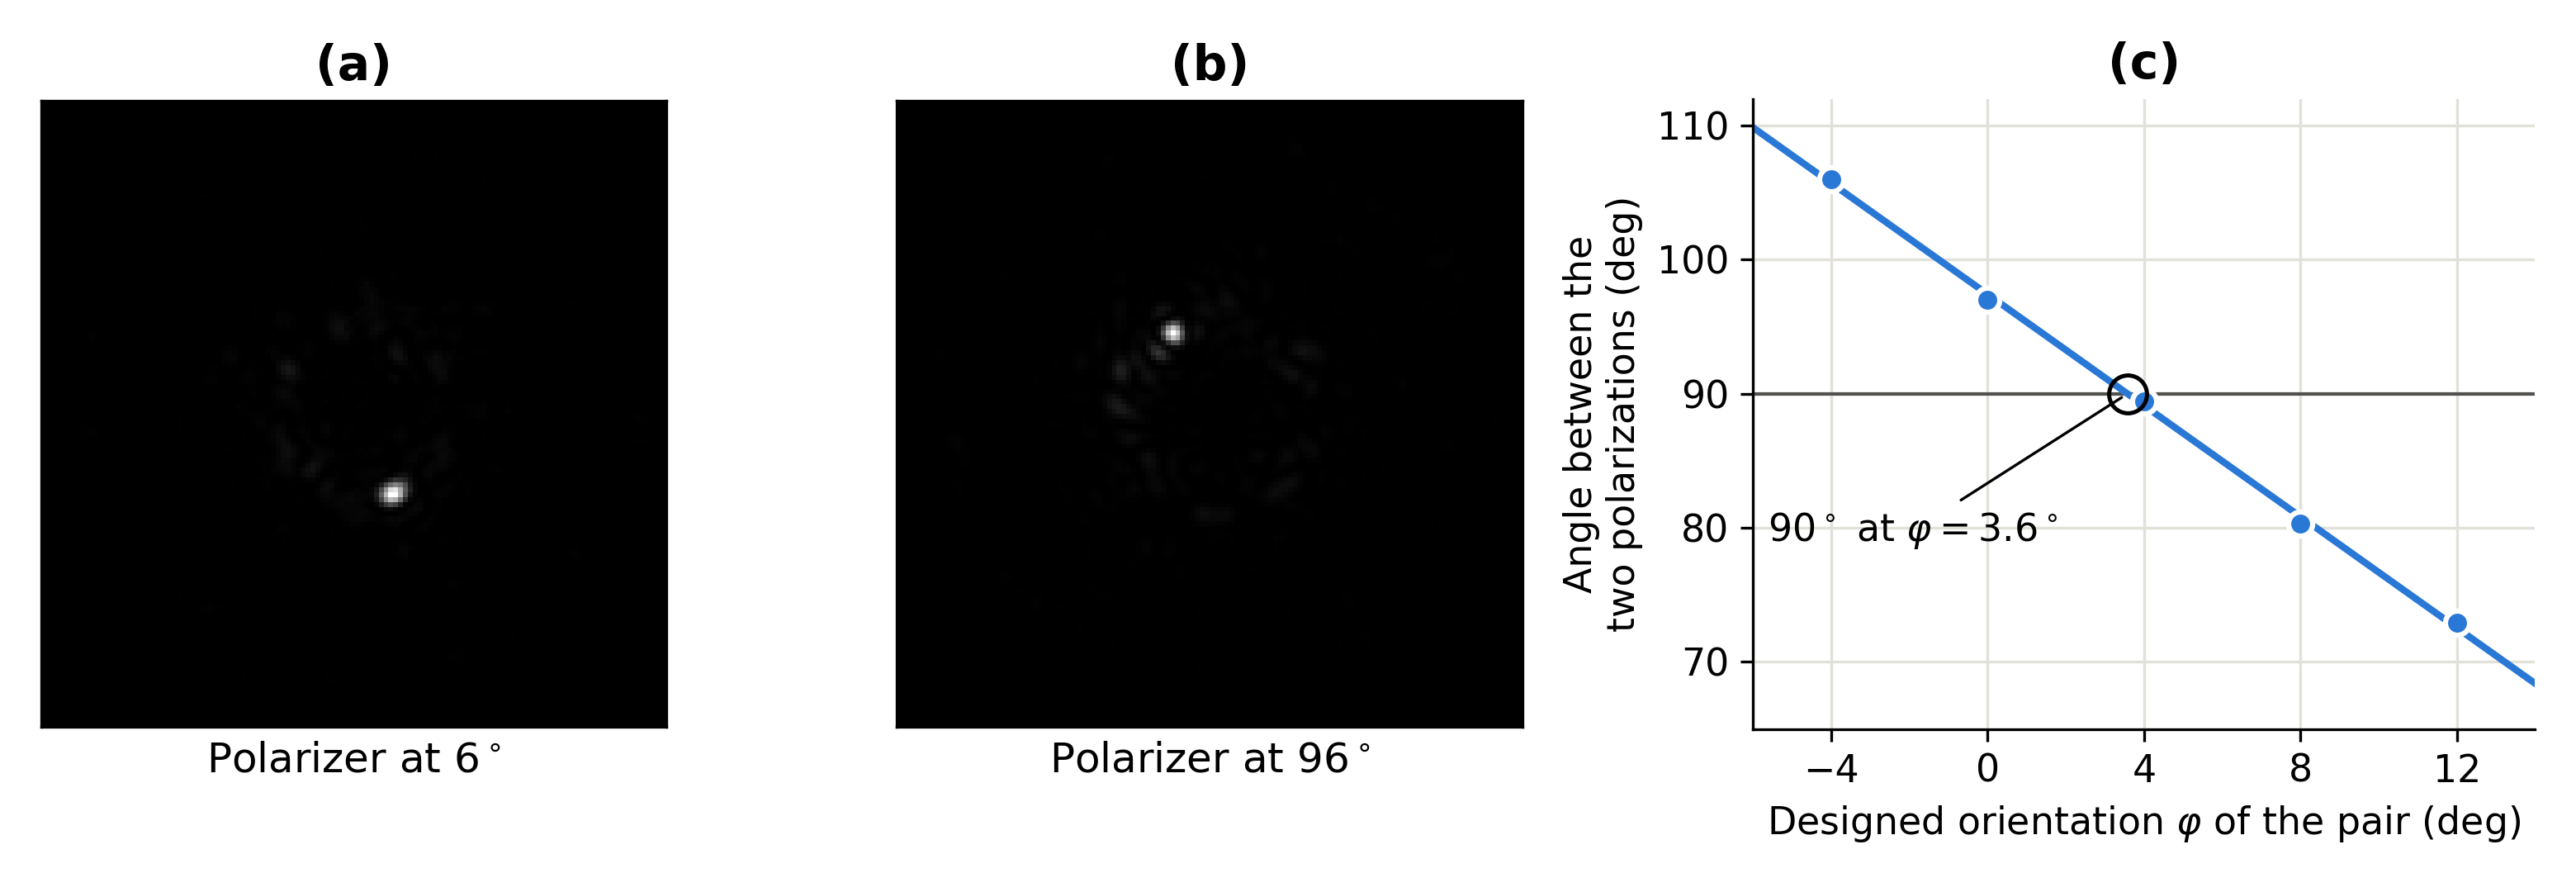
\includegraphics[width=0.95\textwidth]{figures/polarization_axes_experiment.png}
\caption{\textbf{Polarization frame with the camera weight in the forward model.} (a,b) Fourier-plane camera images of one SLM pattern, designed with the retrieved TM alone for a focus A polarized along $x'$ (upper left) and a focus B polarized along $y'$ (lower right). The polarizer in front of the camera is at stage angles of $6^\circ$ and $96^\circ$. Each image is normalized to its maximum (exposure $192\,\mu$s). (c) Angle between the two polarizations of five pairs of orthogonal, linearly polarized foci, measured behind the unequal weights, against the designed orientation of the pair. The line is a linear fit.}
\label{fig:polexp}
\end{figure}

\paragraph{Experiment.}
We tested Eq.~\eqref{eq:camweights} on a separate recording of the 6032 probe patterns, made with no polarizer in the detection path.
The joint fit of Section~\ref{sec:jointfit} was run for 200 epochs with $b$ as an additional parameter, starting from $b=0.47$, $-0.47$, and $0$.
The three runs converged to $|b|=0.701$, within $0.0002$; the sign only selects which component is labelled $x'$.
Compared with a fit with $b=0$ and otherwise identical settings, the held-out PCC rose from $0.915$ to $0.956$ in the image plane and from $0.931$ to $0.974$ in the Fourier plane.
The three retrieved TMs have the same polarization axes, within $0.1^\circ$ on the Poincar\'e sphere, and differ only in the phase between $x'$ and $y'$.
The axes of two TMs fitted with $b=0$ lie $48^\circ$ and $80^\circ$ away from them on the sphere, as Eq.~\eqref{eq:frame} allows.
The fitted $b$ exceeds the typical value of $0.47$ and lies at the upper end of the range over one fringe.

For verification only, we then placed a linear polarizer on a motorized rotation stage in front of the Fourier-plane camera.
All angles below are stage angles.
First, we recorded 104 SLM patterns behind the polarizer at $0^\circ$, $45^\circ$, $90^\circ$, and $135^\circ$.
We fitted Eq.~\eqref{eq:stokesmodel} to these images, extended by the two weights of Eq.~\eqref{eq:camweights}.
The fitted $U$ was diagonal: the cross terms carried $0.01\%$ of the power, and the ellipticity angle of the $x'$ state was $0.0^\circ$.
The fitted weights correspond to $|b|=0.706$.
The images at $45^\circ$ and $135^\circ$ of all 104 patterns gave $\delta=-42.7^\circ$, and $-42.6^\circ$ and $-42.7^\circ$ for the two halves of the patterns.
Two foci designed with this phase to be linearly polarized at $45^\circ$ and $135^\circ$ at the polarizer had $99.9\%$ and $0.4\%$ of their power at $45^\circ$, at the short exposure.
\note{to be added: $\delta$ from single images at $45^\circ$ of the 104 recorded patterns (offline analysis on the lab PC)}

Second, we optimized one SLM pattern for a focus A polarized along $x'$ and a focus B polarized along $y'$, using the retrieved TM alone.
We measured the power of each focus in its $3\times3$-pixel window behind the polarizer at $6^\circ$ and at $96^\circ$, and denote by $\tau$ the share recorded at $6^\circ$.
The shares were $\tau_A=0.1\%$ and $\tau_B=96.9\%$, a difference of $0.968$.
The blocked focus was evaluated at an exposure 32 times longer than that of the transmitted one, at which it lies above the dark level of the camera.
The polarizer extinguished focus A at $4.5^\circ\pm0.2^\circ$ and focus B at $99.1^\circ\pm0.7^\circ$.
The minimum of focus B was $3.6\%$ of its maximum, which bounds its ellipticity in front of BS2 to about $4.5^\circ$.
For a TM fitted with $b=0$, the same test at $0^\circ$ and $90^\circ$ gave a difference of $0.70$, and one focus was elliptically polarized (degree of linear polarization $0.72$).

Third, we located the axes of Eq.~\eqref{eq:camweights} on the stage scale.
Unequal weights preserve the angle between two orthogonal linear states only if the states lie on the axes of the weights.
We designed five pairs of orthogonal, linearly polarized foci whose common orientation was stepped over $16^\circ$.
The measured angle between the two polarizations of a pair fell from $106.0^\circ$ to $72.9^\circ$ and crossed $90^\circ$ where the pair lay at $4.9^\circ$ and $94.9^\circ$ ($\pm0.2^\circ$).
With the weights removed, $x'$ and $y'$ lie at $94.1^\circ$ and $6.6^\circ$, within $2^\circ$ of these axes.
A fit of the weights to the ten measured orientations gave $|b|=0.737\pm0.006$.
Finally, a fixed polarizer, aligned by hand with a laboratory axis, was parallel to the rotating polarizer at $95.1^\circ$.
The axes of Eq.~\eqref{eq:camweights} thus agree with the laboratory axes within the accuracy of this alignment.
Figure~\ref{fig:polexp} shows the two foci and the pairs, and Table~\ref{tab:polframe} summarizes the results.

\begin{table}[h]
\centering
\caption{\textbf{Polarization frame with the camera weight in the forward model.} Angles are stage angles of the rotating polarizer.}
\label{tab:polframe}
\small
\begin{tabular}{p{0.31\textwidth}p{0.25\textwidth}p{0.36\textwidth}}
\toprule
Quantity & Expected & Measured \\
\midrule
$|b|$ from the joint fit & $0.47$ (range $0.36$--$0.69$) & $0.701$ (three runs, within $0.0002$) \\
$|b|$ at the polarizer & equal to the fitted value & $0.706$ (speckle), $0.737\pm0.006$ (pairs of foci) \\
Cross-term power of $U$ & $0$ & $0.01\%$ \\
Axes of the weights & laboratory axes & $4.9^\circ$ and $94.9^\circ$; fixed polarizer at $95.1^\circ$ \\
Axes $x'$ and $y'$ & axes of the weights & $94.1^\circ$ and $6.6^\circ$ \\
Share of a focus at its orientation & $100\%$ & $99.9\%$ (A), $96.9\%$ (B) \\
Phase between $x'$ and $y'$ & free & $-42.7^\circ$ \\
\bottomrule
\end{tabular}
\end{table}


\clearpage
\bibliography{references}
\end{document}
